\subsection{Delay offset, subspace width, and useful averaging}
\label{sec:operatingregion}
A prespecified sensitivity study varies the pilot count, delay offset, and
integer-window length. It uses $N=64$, $M\in\{16,32\}$ equally spaced pilots,
delays $(0,7+\delta,11+\delta)$, powers $(0.5,0.3,0.2)$,
$\delta=0,0.1,\ldots,0.9$, and $L=12,13,14,15$.
The 160 combinations of geometry and SNR (10 and 20~dB) are evaluated
analytically for $T=1,4,16$. Independent Monte Carlo checks use 20\,000 groups
per condition at 20~dB for both pilot counts, $L=12,15$, and
$\delta=0,0.2,0.5,0.9$. The complete grid and group estimates are archived.

Figure~\ref{fig:operatingregion} shows how the crossover changes with the
channel geometry. Here normalized calibration MSE means
$\mathbb E[(\widehat v_T-v)^2]/v^2$, distinct from the full-channel NMSE in
Eq.~\eqref{eq:nmse}. At $M=16$, $\delta=0.5$, and 20~dB, increasing $L$ from
12 to 15 reduces $b/v$ from 40.79 to 5.00 and normalized calibration MSE
at $T=16$ from 1765.78 to 27.24. The corresponding $T_\star$ values are
0.98 and 1.44 blocks: both estimates are bias-dominated well before 16
independent blocks. With 32 pilots, the same window change reduces normalized
MSE from 333.46 to 7.31. Across the 48 Monte Carlo checks (16 conditions,
three block counts), means and mean-square errors differ from their predictions
by at most 2.91 and 2.79 Monte Carlo standard errors; sample variances differ
by at most 3.02\%.

\begin{figure}[t]
\centering
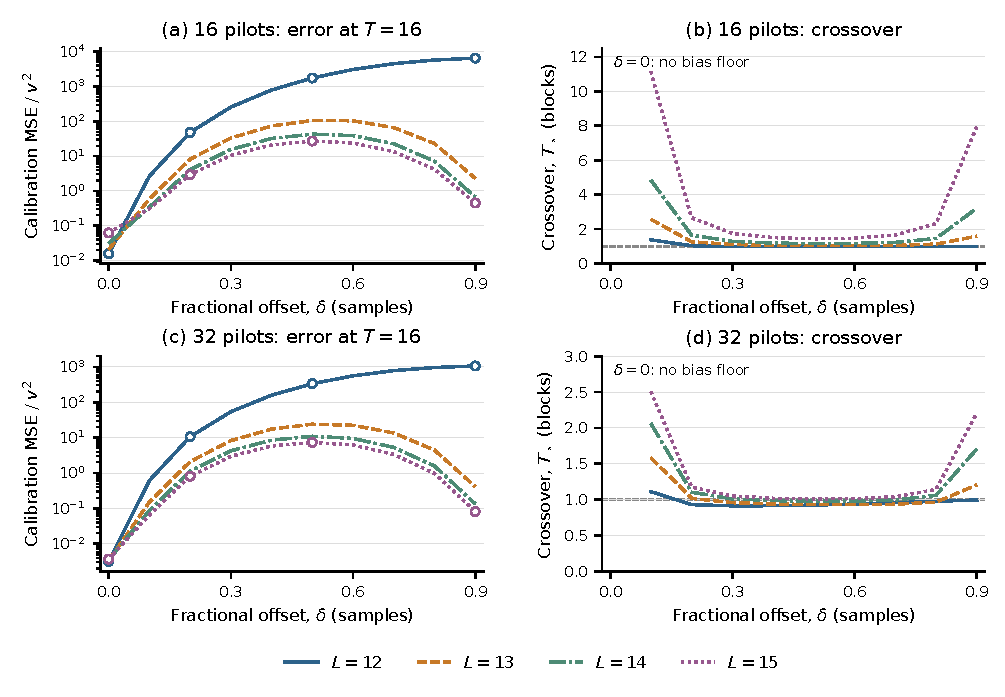
\includegraphics[width=\linewidth]{operating_region.pdf}
\caption{Geometry and window sensitivity at 20~dB with independent gains.
Left: normalized calibration MSE at $T=16$; curves give the analytical
grid and open circles the Monte Carlo checks for $L=12,15$ (20\,000 groups
per condition). Right: the bias--variance crossover $T_\star$ for nonzero
offsets. At $\delta=0$, the channel lies in every tested subspace and there
is no finite crossover. The dashed horizontal reference marks one block.
Lines connect evaluated offsets; the full archive also contains 10~dB and
$T=1,4$ results.}
\label{fig:operatingregion}
\end{figure}

Wider windows reduce both raw leakage and normalized bias at every fractional
offset in this grid, but the calibration MSE also depends on the remaining
residual dimensions. At $M=16$, $\delta=0.1$, and 10~dB, changing $L$ from
12 to 15 lowers $b/v$ from 0.157 to 0.043 while increasing normalized MSE
at $T=16$ from 0.0465 to 0.0698. The intermediate choice $L=13$ gives
0.0292, the smallest MSE among the four tested widths in this condition.
For the matched integer case, the same
change increases MSE from $1/64$ to $1/16$. Thus a wider window is beneficial
when the leakage reduction compensates for the variance cost. The crossover
and MSE quantify that trade-off for the specified channel family and noise level.
